\documentclass{beamer}
\usetheme{afm}

\title{Interest Rate and\\\vspace{0.25cm}Credit Derivatives}
\author{Matteo Sani - \href{mailto:matteo.sani@unisi.it}{matteo.sani@unisi.it}}

\begin{document}
\begin{frame}[plain]
	\maketitle
\end{frame}

\begin{frame}{Interest Rate Swaps}
	\begin{itemize}
		\item \emph{Interest rate swaps} (IRS) consist of a floating leg and a fixed leg. The contract parameters are:
		\begin{itemize}
		\item start date $d_0$;
		\item notional $N$;
		\item fixed rate $K$;
		\item floating rate tenor;
		\item maturity.
		\end{itemize}
		\item \emph{Floating leg}: pays the reference IBOR fixing at a frequency equal to the index tenor (e.g. an IRS on a 3-month EURIBOR will pay coupons every three months).
		\item \emph{Fixed leg}: pays a predetermined cash flow at annual frequency (for simplicity only consider maturities multiples of 1 year).
	\end{itemize}
\end{frame}

\begin{frame}{IRS Valuation}
	\begin{itemize}
		\item The NPV of the fixed leg is calculated as follows:
		\begin{equation*}
		\mathrm{NPV}_{\mathrm{fixed}}(d, K) = N\cdot K\cdot\sum_{i=1}^{n}D(d, d_{i}^{\mathrm{fixed}})
		\end{equation*}
		\item While the NPV of the floating leg is:
		\begin{equation*}
			\mathrm{NPV}_{\mathrm{float}}(d, F) = N\cdot\sum_{i=1}^{m}F(d, d_{j-1}^{\mathrm{float}}, d_{j}^{\mathrm{float}}) \cdot \tau
\cdot D(d, d_{i}^{\mathrm{float}})
		\end{equation*}
		where $d_i^{\mathrm{fixed}}, d_i^{\mathrm{float}}$ are the payment dates, $d$ the pricing date, $D(d, d')$ the discount factor between $d$ and $d'$, $F(d, d', d'')$ the forward rate and $\tau = \frac{d_{j}^{\mathrm{float}}-d_{j-1}^{\mathrm{float}}}{360}$ the tenor.		
		\item Therefore the NPV of the swap (seen from the point of view of the counter-party which receives the floating leg) is
		\begin{equation*}
			\mathrm{NPV}(d, F, K) = \mathrm{NPV}_{\mathrm{float}}(d,F) - \mathrm{NPV}_{\mathrm{fixed}}(d,K)
		\end{equation*} 
	\end{itemize}
\end{frame}
	
\begin{frame}{IRS Valuation}
	\begin{itemize}	
	\item It's actually more convenient to express the NPV as a function of the \emph{swap rate} $S$.
	\item $S$ is the value of $K$ which makes $\mathrm{NPV}=0$ or 		$\mathrm{NPV}_{\mathrm{fixed}}(d, S) = \mathrm{NPV}_{\mathrm{float}}(d, F)$.
	\begin{equation*}
		\begin{gathered}
		N\cdot S\cdot\sum_{i=1}^{n}D(d, d_{i}^{\mathrm{fixed}}) = N\cdot\sum_{i=1}^{m}F(d, d_{j-1}^{\mathrm{float}}, d_{j}^{\mathrm{float}}) \cdot\tau\cdot D(d, d_{i}^{\mathrm{float}})\\
		S=\frac{\sum_{i=1}^{m}F(d, d_{j-1}^{\mathrm{float}}, d_{j}^{\mathrm{float}}) \cdot \tau\cdot D(d, d_{i}^{\mathrm{float}})}{\sum_{i=1}^{n}D(d, d_i^{\mathrm{fixed}})}
		\end{gathered}
	\end{equation*}
	\item Once calculated $S$, we can write:
	\begin{align*}
	&\mathrm{NPV} = \mathrm{NPV}_{\mathrm{float}}(d, F) - \mathrm{NPV}_{\mathrm{fixed}}(d, K) = \overbrace{\mathrm{NPV}_{\mathrm{float}}(d, F) - \mathrm{NPV}_{\mathrm{fixed}}(d, S)}^{\mathrm{=\;0}} + \\& + \mathrm{NPV}_{\mathrm{fixed}}(d, S) - \mathrm{NPV}_{\mathrm{fixed}}(d, K) = N\cdot(S-K)\cdot\underbrace{\sum_{i=1}^{n}D(d, d_{i}^{\mathrm{fixed}})}_{\mathrm{annuity}}
	\end{align*}
	\end{itemize}
\end{frame}

\begin{frame}{Interest Rate Swaptions}
	\begin{itemize}
		\item \emph{Swaptions} (Swap-options) are the equivalent of European options for the interest rate markets.
		\item They give the holder the right but not the obligation, at the exercise date $d_{ex}$, to enter into an Interest Rate Swap at a pre-determined fixed rate.
		\item The holder will choose to exercise the option only if the NPV of the underlying swap at $d_{ex}$ will be positive.
		\item From the IRS NPV expression, we can determine the payoff of the swaption 
		\begin{equation*}
		N\cdot \mathrm{max}(0, S(d_{\mathrm{ex}}) - K)\cdot\sum D(d, d_i^{\mathrm{fixed}})
		\end{equation*}
		\item In order to valuate the swaption the key point is to estimate $S(d_{\mathrm{ex}})$. 
		\item It will be shown with two alternative approaches.
	\end{itemize}
\end{frame}

\begin{frame}{Swaption Price with Black-Scholes}
    \begin{itemize}	
    \item First we'll use a generalization of the Black-Scholes formula for swaptions:
    \begin{equation*}
    \mathrm{NPV} = N\cdot A\cdot [S \Phi(d_+) - K\Phi(d_-)]
    \end{equation*}
    where $\Phi$ represents the cumulative distribution function of the normal distribution
    \begin{gather*}
    d_{\pm} = \frac{\mathrm{log}(\frac{S}{K}) \pm \frac{1}{2}\sigma^{2}T}{\sigma\sqrt{T}}\qquad(\sigma~\textrm{is the volatility of the swap rate})\\
    A =\sum_{i=1}^{p}D(d, d_{i}^{\mathrm{fixed}})\qquad\mathrm{(annuity})
    \end{gather*}
    \end{itemize}
\end{frame}

\begin{frame}{Swaption Price with Monte Carlo}
    \begin{itemize}
    \item An alternative approach is to assume that the swap rate $S$ evolves following a log normal process.
    \item Its distribution at the exercise date $S(d_{\mathrm{ex}})$ is
    \begin{equation*}
    S(d)\mathrm{exp}\left[-\frac{1}{2}\sigma^{2}T+\sigma\sqrt{T}\mathcal{N}(0,1)\right]	
    \end{equation*} 
	notice that the \emph{drift} rate in the evolution is zero.
    \item To simulate the swap rate we can:
    \begin{enumerate}
    \item sample $n$ times from the normal distribution $\mathcal{N}(0, 1)$ and calculate $S(d_{\mathrm{ex}})$ in different scenrios;
    \item evaluate the underlying swap's NPV at the exercise date, and consequently the swaption's payoff, for each scenario;
    \item take the average of these values to get the final estimate.
  	\end{enumerate} 
  	\item Further the 95\% confidence level for the swaption simulation can be calculated to compare with the BS result.
    \end{itemize}
\end{frame}

\begin{frame}{Credit Curves}
\begin{itemize}
    \item A \emph{credit event} can be a default, the failure to make payments, the issuer entering into bankruptcy proceedings, or the occurence of other legal events\dots (for simplicity credit event = default).
    \item \emph{Non-default probability} or \emph{survival probability} ($P_{\textrm{sur}}$): probability that the issuer of a contract will not suffer a credit event before a given date. 
    \item Note that non-default probability is a \emph{cumulative probability} since refers to a certain time horizon. 
    \item Just like a discount curve is a way of representing a set of discount factors, \emph{credit curves} are a way of representing survival probabilities.
\end{itemize}
\end{frame}

\begin{frame}{Hazard Rate}
	\begin{itemize}
		\item \emph{Hazard rate} measures the instantaneous probability of a company defaulting \emph{conditioned} on it not having defaulted until that moment.
		\item Hazard rate is often called a \emph{conditional failure rate} since is a direct application of the conditional probability concept (i.e. tells "how should you update probabilities of events when there is additional information available"). 
		\begin{equation*}
		\lambda(t) = -\cfrac{dP_{\textrm{sur}}}{dt}\cfrac{1}{P_{\textrm{sur}}(t_0, t)}
		\end{equation*}
		where the minus sign derives from the fact that $P_{\textrm{sur}}$ is a \emph{non} default probability while the hazard rate is defined in terms of the probability of default $P_{\textrm{def}}$.
	\end{itemize}
\end{frame}

\begin{frame}{Hazard Rate}
	\begin{itemize}
		\item Given the hazard rate the survival probability can be determined as:
		\begin{gather*}
		\lambda(t) = -\cfrac{1}{dt}\cdot\cfrac{dP_{\textrm{sur}}}{P_{\textrm{sur}}} = -\cfrac{d(\textrm{log}P_{\textrm{sur}})}{dt}\\[5pt]
		P_{\textrm{sur}}(t_0, t) = e^{-\int_{t_0}^{t}\lambda(s) ds}
		\end{gather*}
		
		\item For example a constant hazard rate results in the following probabilities:
		\begin{gather*}
			P_{\textrm{sur}}(t_0, t) = e^{-\lambda (t-t_0)}\\
			P_{\textrm{def}}(t_0, t) = 1 - e^{-\lambda (t-t_0)}
		\end{gather*}
	\end{itemize}
\end{frame}

\begin{frame}{Credit Default Swap}
\begin{itemize}
\item A Credit Default Swap (CDS) is a financial agreement where the seller compensate the buyer in case of a credit event of a reference asset.
\item In other words, the seller of the CDS \emph{insures} the buyer against possible credit events.
\item To get such \emph{protection} the CDS buyer makes a series of payments (the "spread") to the seller and, in exchange, may expect to receive a payoff if the asset defaults. 
\item CDSs are made up of two legs:
\begin{itemize}
    \item \emph{default leg}: which pays $LGD = F(1 - R)$ if and when the credit event occurs ($LGD$ is the \emph{loss given default}, $F$ the face value of the contract and $R$ is the recovery rate usually set around 40\%);
    \item \emph{premium leg}: which pays the \emph{spread} $S$ every $m$ months until the credit event occurs or the contract expires.
\end{itemize}
\end{itemize}
\end{frame}

\begin{frame}{CDS Valuation}
\begin{itemize}
\item Given the following contract characteristics:
\begin{itemize}
\item $d$ today's date;
\item $d_0$ the start date of the CDS (could be different from $d$);
\item $d_1, ..., d_n$ the payment dates of the premium leg, which occur at a m-month frequency (we assume that $d_n$ is the end date of the CDS);
\item $D(d')$ the discount factor between $d$ and $d'$;
\item $P_{\textrm{sur}}(d')$ the survival probability between $d$ and $d'$;
\item $\tau$ the random variable representing the date of the credit event.
\end{itemize}
CDS can be priced as
\begin{align*}
\textrm{NPV}_{\textrm{premium}} &= F\cdot S\cdot \sum_{i=1}^{n} D(d_i) \cdot P_{\textrm{sur}}(d_i) \\
\mathrm{NPV_{default}} &= F(1-R) \sum_{d'=d_0}^{d_n} D(d') \left( P_{\textrm{sur}}(d') - P_{\textrm{sur}}(d'+1) \right)
\end{align*}
\end{itemize}
\end{frame}

\begin{frame}{Default Probability from Bond Prices}
\begin{itemize}
\item Bond price is directly linked to the credit rating of the issuer, i.e. the associated default risk implies the borrower might not be able to repay the loan.
\begin{itemize}
    \item Bonds with low ratings (\emph{junk bonds}) are sold at lower prices since riskier;
    \item high ratings bonds (\emph{investment-grade bonds}) are sold at higher prices.
\end{itemize}
\item The average hazard rate can be approximated by considering the spread $s$ between a risky bond yield and the risk-free rate, and $R$ the recovery rate. 
\item The bond value $e^{-(r+s)\cdot T}$ can also be expressed in terms of default probability (or hazard rate)
\begin{equation*}
e^{-(r+s)\cdot T} = 
\begin{cases}
R\;\;\textrm{with probability}\;1 - e^{-\lambda T} \\
1\;\;\textrm{with probability}\;e^{-\lambda T} \\
\end{cases} = 
(e^{-\lambda T} + R - R e^{-\lambda T})e^{-rT}
\end{equation*}
where the hazard rate has been assumed constant.
\end{itemize}
\end{frame}

\begin{frame}{Default Probability from Bond Prices}
\begin{itemize}
\item If $\lambda$ is small, from a Taylor expansion we get $e^{x} = 1 + x + \mathcal{O}(x^2)$ so
\begin{equation*}
\begin{gathered}
\cancel{e^{-rT}}e^{-sT}= (e^{-\lambda T} + R - R e^{-\lambda T})\cancel{e^{-rT}} \\
\cancel{1} - s\cancel{T} = \cancel{1} - \lambda \cancel{T} + \cancel{R} - \cancel{R} + R\lambda \cancel{T} \\
s = (1 - R)\cdot \lambda \implies \bar{\lambda} = \frac{s}{1-R}
\end{gathered}
\end{equation*}
\item Imagine a bond that yields 150 basis points more than a similar risk-free bond and assume an expected recovery rate of 40\%.
\begin{equation*}
\bar{\lambda} = \cfrac{0.015}{(1-0.4)} = 2.5\%
\end{equation*}
\end{itemize}
\end{frame}

\begin{frame}{Default Probability from CDS}
\begin{itemize}
\item With bootstrapping it is possible to derive survival probabilities from credit curve.
\item The technique is analogous to that used with discount curve to get discount factors
\begin{enumerate}
\item collect market quotes for a number of CDS with different maturities;
\item create the corresponding CDS objects;
\item define a credit curve whose pillars are the CDS maturity dates and the survival probabilities are unknown;
\item define an objective function to minimize the sum of the squared CDS's NPVs;
\item set the non-default probabilities to an initial value and define their range of variability between [0, 1] since they are probabilities and fix "today's" probability to 1 since there hasn't been any default;
\item run the minimization.
\end{enumerate}
\end{itemize}
\end{frame}

\begin{frame}{Credit Suisse Example (2022-09-29)}
"\textit{This morning Credit Suisse reached its minimum of 3.52 CHF (-11,5\%)...After Archegos and Greensill scandals analysists says three options are left: CS could straighten up by itself (a "miracle"), could be acquired by another bank or saved by Swiss Governament aids.}"
\begin{figure}[h]
    \begin{center}
    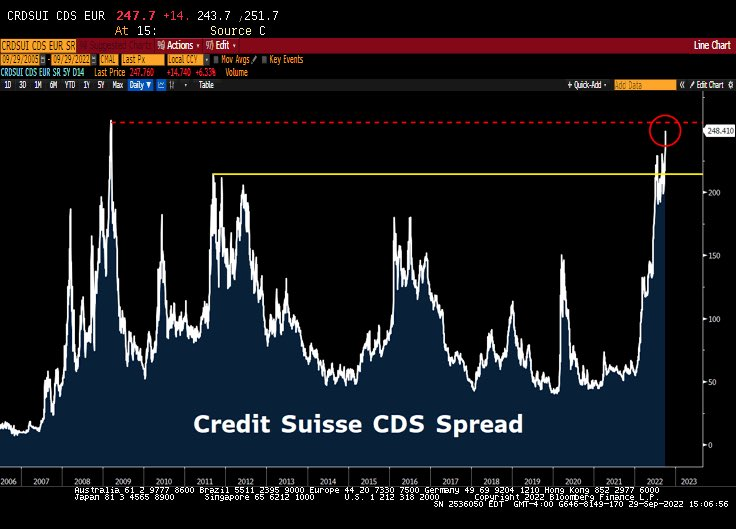
\includegraphics[width=0.45\linewidth]{cds_credit_suisse}\quad
    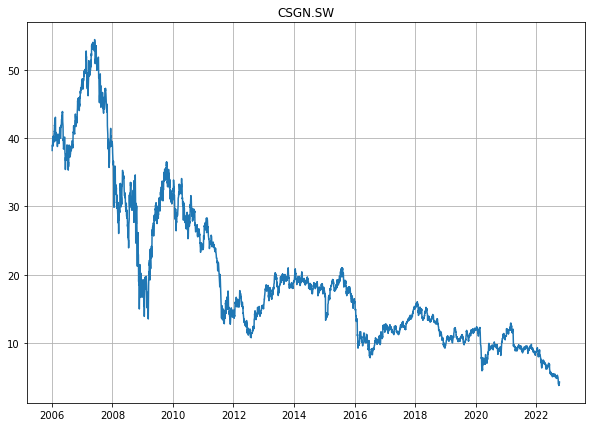
\includegraphics[width=0.45\linewidth]{price_credit_suisse}
    \end{center}
\end{figure}    
\end{frame}

\begin{frame}[fragile]{Credit Suisse Example (2022-09-29)}
\begin{ipython}
! pip install yfinance
\end{ipython}

\begin{ipython}
import yfinance as yf
from datetime import date
import matplotlib.pyplot as plt

proxy = yf.Ticker('CSGN.SW')
data = proxy.history(start='2006-01-05')['Close']

plt.rcParams['figure.figsize'] = (10, 7)
plt.plot(data)
plt.grid(True)
plt.title("CSGN.SW")
plt.show()
\end{ipython}
\end{frame}
\end{document}
